\documentclass[letter,11pt]{article}

\usepackage[spanish,es-nodecimaldot]{babel}
\usepackage[utf8]{inputenc}

\usepackage{lmodern}
\usepackage[T1]{fontenc}
\usepackage{textcomp}

\usepackage{framed}
\usepackage[svgnames]{xcolor}
\colorlet{shadecolor}{Gainsboro!50}

\usepackage{graphicx}
\usepackage{pstricks}

\usepackage{anysize}
\marginsize{3cm}{2cm}{2cm}{3cm}

\usepackage{siunitx}
\usepackage{amsmath}
\usepackage{array}

\usepackage{fancyhdr}
\usepackage{lastpage}
\pagestyle{fancy}
\fancyhf{}
\fancyhead[LE,RO]{Laboratorio de Física Básica III}
\fancyfoot[CO,CE]{\thepage\ de \pageref{LastPage}}

\special{papersize=215.9mm,279.4mm}

\usepackage[
    pdfauthor={Carlos Eduardo Caballero Burgoa},%
    pdftitle={Laboratorio de Física Básica III},%
    pdfsubject={1er Parcial},%
    colorlinks,%
    citecolor=black,%
    filecolor=black,%
    linkcolor=black,%
    urlcolor=black,
    breaklinks]{hyperref}
\usepackage{breakurl}

\newcommand{\blankpage}{
\newpage
\thispagestyle{empty}
\mbox{}
\newpage
}

\renewcommand{\arraystretch}{1.2}

\begin{document}

\begin{center}
    {\Large \bf{Primer parcial}}
\end{center}

\noindent\fbox{%
    \parbox{\textwidth}{%
        Estudiante: CABALLERO BURGOA, Carlos Eduardo \\
        Carrera: Ingeniería Electromecánica \\
        Correo: cijkb.j@gmail.com
    }%
}

\vspace{1.0cm}

\begin{enumerate}
\item A partir de la siguiente tabla, determinar la resistencia interna (con su
    error), la corriente de corto circuito (sin su error) y la FEM (con su
    error).

    \begin{center}
    \begin{tabular}{|c|c|c|c|c|c|c|c|c|c|c|}
    \hline
    No. & 1 & 2 & 3 & 4 & 5 & 6 & 7 & 8 & 9 & 10 \tabularnewline \hline
    $I[mA]$ & 30 & 34 & 38 & 42 & 46 & 50 & 54 & 58 & 62 & 66 \tabularnewline \hline
    $V[V]$  & 2.8 & 2.79 & 2.76 & 2.72 & 2.70 & 2.68 & 2.66 & 2.64 & 2.64 & 2.60 \tabularnewline \hline
    \end{tabular}
    \end{center}

    Solución: \\
    Se obtiene el siguiente gráfico:

    \begin{figure}[!h]
    \centering
    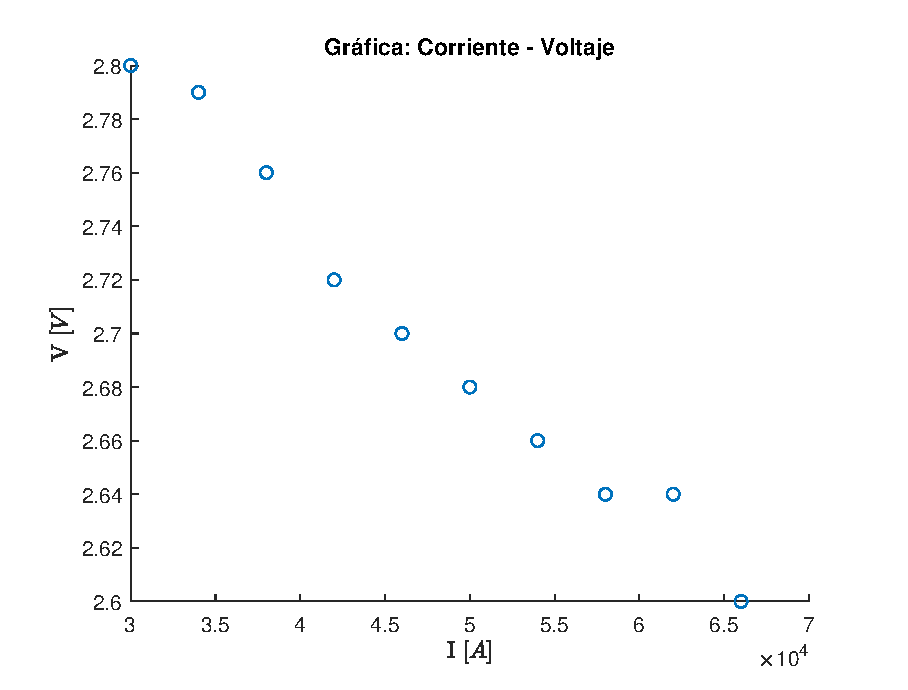
\includegraphics[scale=0.75]{resources/m1.eps}
    \end{figure}

    Por tanto, la ecuación de ajuste es:

    \begin{equation*}
        V_{ab} = A + B \cdot I
    \end{equation*}

    Calculamos los parámetros de la recta por el método de los mínimos cuadrados,
    con la ayuda de los datos presentados.

    \begin{tabular}{|c|>{\centering}m{1.6cm}<{\centering}
                      |>{\centering}m{1.6cm}<{\centering}
                      |>{\centering}m{1.6cm}<{\centering}|
                      |>{\centering}m{1.6cm}<{\centering}
                      |>{\centering}m{1.6cm}<{\centering}
                      |>{\centering}m{1.6cm}<{\centering}|}
    \hline
    $i$ & $I^2_i$ & $V^2_i$ & $I_i V_i$ & $Y$ & $d_i$ & $d^2_i (\num{e-3})$ 
        \tabularnewline \hline \hline
     1 & 0.0009 & 7.8400 & 0.0840 & 2.7985 &  0.0015 & 0.0021 \tabularnewline \hline
     2 & 0.0012 & 7.7841 & 0.0949 & 2.7764 &  0.0136 & 0.1843 \tabularnewline \hline
     3 & 0.0014 & 7.6176 & 0.1049 & 2.7543 &  0.0057 & 0.0325 \tabularnewline \hline
     4 & 0.0018 & 7.3984 & 0.1142 & 2.7322 & -0.0122 & 0.1484 \tabularnewline \hline
     5 & 0.0021 & 7.2900 & 0.1242 & 2.7101 & -0.0101 & 0.1012 \tabularnewline \hline
     6 & 0.0025 & 7.1824 & 0.1340 & 2.6879 & -0.0079 & 0.0630 \tabularnewline \hline
     7 & 0.0029 & 7.0756 & 0.1436 & 2.6658 & -0.0058 & 0.0339 \tabularnewline \hline
     8 & 0.0034 & 6.9696 & 0.1531 & 2.6437 & -0.0037 & 0.0137 \tabularnewline \hline
     9 & 0.0038 & 6.9696 & 0.1637 & 2.6216 &  0.0184 & 0.3395 \tabularnewline \hline
    10 & 0.0044 & 6.7600 & 0.1716 & 2.5995 &  0.0005 & 0.0003 \tabularnewline \hline
    \end{tabular}

    \begin{equation*}
        n = 10
    \end{equation*}
    \begin{equation*}
        \sum I_i = 0.4800
    \end{equation*}
    \begin{equation*}
        \sum V_i = 26.9900
    \end{equation*}
    \begin{equation*}
        \sum I^2_i = 0.0244
    \end{equation*}
    \begin{equation*}
        \sum V^2_i = 72.8873
    \end{equation*}
    \begin{equation*}
        \sum I_i V_i = 1.2882
    \end{equation*}
    \begin{equation*}
        \Delta_1 = n \sum I^2_i - \left( \sum I_i \right)^2 = 0.0132
    \end{equation*}
    \begin{equation*}
        \Delta_2 = n \sum V^2_i - \left( \sum V_i \right)^2 = 0.4129
    \end{equation*}
    \begin{equation*}
        A = \frac{\sum V_i \sum I^2_i - \sum I_i V_i \sum I_i}{\Delta_1} = 2.9645
    \end{equation*}
    \begin{equation*}
        B = \frac{n \sum I_i V_i - \sum I_i \sum V_i}{\Delta_1} = -5.5303
    \end{equation*}
    \begin{equation*}
        \sum d^2 = \num{9.1879e-4}
    \end{equation*}
    \begin{equation*}
        \sigma^2 = \frac{\sum d^2_i}{n-2} = \num{1.1485e-4}
    \end{equation*}
    \begin{equation*}
        \sigma_A = \sqrt{\frac{\sigma^2 \sum d^2_i}{\Delta_1}} = 0.0146
    \end{equation*}
    \begin{equation*}
        \sigma_B = \sqrt{\frac{\sigma^2 n}{\Delta_1}} = 0.2950
    \end{equation*}

    \begin{equation*}
        A = (2.96 \pm 0.01)[V]; 0.49 \%
    \end{equation*}
    \begin{equation*}
        B = (-5.5 \pm 0.3)[\Omega]; 5.33 \%
    \end{equation*}

    Siendo el coeficiente de correlación:

    \begin{equation*}
        r = \frac{n \sum I_i V_i - (\sum I_i)(\sum V_i)}{\sqrt{\Delta_1 \Delta_2}} = -0.9888
    \end{equation*}

    La ecuación de la recta resultante es:

    \begin{equation*}
        V_{ab} = 2.96 - 5.5\, I
    \end{equation*}

    \begin{center}
    \begin{tabular}{|>{\centering}m{11.0cm}<{\centering}|}
    \hline
    \textbf{Resultado}
    \tabularnewline \hline
    \\
    $\varepsilon = (2.96 \pm 0.01) [V]; 0.49 \%$ \tabularnewline
    \\
    \hline
    \end{tabular}
    \end{center}

    \begin{center}
    \begin{tabular}{|>{\centering}m{11.0cm}<{\centering}|}
    \hline
    \textbf{Resultado}
    \tabularnewline \hline
    \\
    $r_i = (5.5 \pm 0.3) [\Omega]; 5.33 \%$ \tabularnewline
    \\
    \hline
    \end{tabular}
    \end{center}

    Por tanto:

    \begin{center}
    \begin{tabular}{|>{\centering}m{11.0cm}<{\centering}|}
    \hline
    \textbf{Resultado}
    \tabularnewline \hline
    \\
    $I_{cc} = \frac{\epsilon}{r_i} = 0.54 [A]$ \tabularnewline
    \\
    \hline
    \end{tabular}
    \end{center}

\newpage
\item A partir de los siguientes datos determinar la constante de la
    permisividad del vacío con su respectivo error. Considere las cargas iguales
    a: $4.2 [\mu C]$ y $7.89 [\mu C]$.

    \begin{center}
    \begin{tabular}{|c|c|c|c|c|c|}
    \hline
    No. & 1 & 2 & 3 & 4 & 5 \tabularnewline \hline
    $d[m]$ & 0.02 & 0.03 & 0.04 & 0.05 & 0.06 \tabularnewline \hline
    $F[N]$ & 719.0 & 320.1 & 179.9 & 115.0 & 80.0 \tabularnewline \hline
    \end{tabular}
    \end{center}

    Solución: \\
    Se obtiene el siguiente gráfico:

    \begin{figure}[!h]
    \centering
    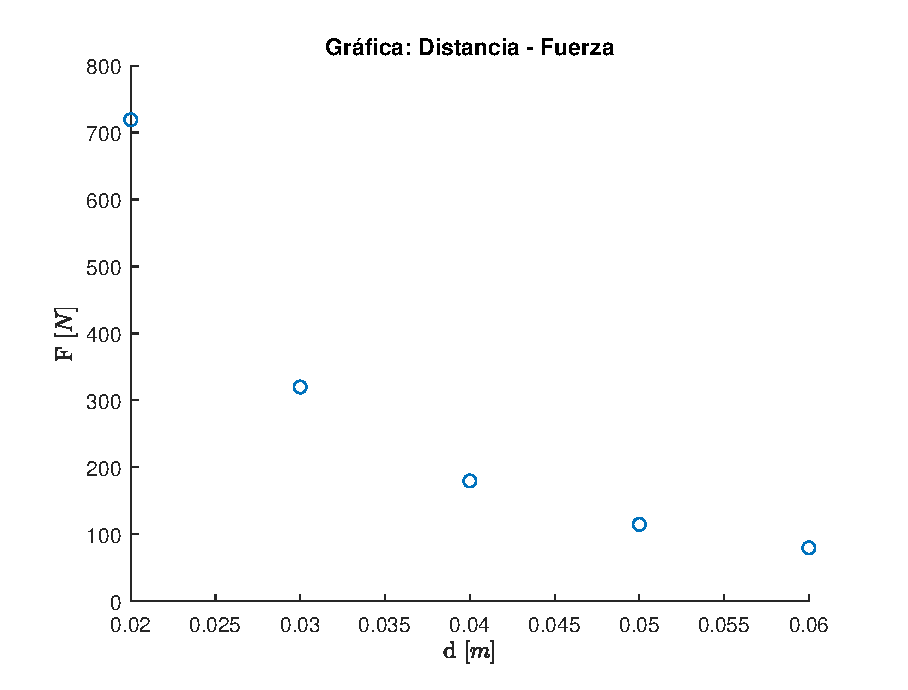
\includegraphics[scale=0.75]{resources/m2.eps}
    \end{figure}

    Por tanto, la ecuación de ajuste es:

    \begin{equation*}
        F = a x^b
    \end{equation*}

    Linealizando los valores:

    \begin{center}
    \begin{tabular}{|c|c|c|c|c|c|}
    \hline
    No. & 1 & 2 & 3 & 4 & 5 \tabularnewline \hline
    $ln(d)$ & -3.9120 & -3.5066 & -3.2189 & -2.9957 & -2.8134 \tabularnewline \hline
    $ln(F)$ & 6.5779 & 5.7696 & 5.1924 & 4.7449 & 4.3820 \tabularnewline \hline
    \end{tabular}
    \end{center}

    Calculamos los parámetros de la recta por el método de los mínimos cuadrados,
    con la ayuda de los datos presentados.

    \begin{tabular}{|c|>{\centering}m{1.6cm}<{\centering}
                      |>{\centering}m{1.6cm}<{\centering}
                      |>{\centering}m{1.6cm}<{\centering}|
                      |>{\centering}m{1.6cm}<{\centering}
                      |>{\centering}m{1.6cm}<{\centering}
                      |>{\centering}m{1.6cm}<{\centering}|}
    \hline
    $i$ & $d^2_i$ & $F^2_i$ & $d_i F_i$ & $Y$ & $\delta_i$ & $\delta^2_i (\num{e-5})$ 
        \tabularnewline \hline \hline
     1 & 15.3039 & 43.2683 & -25.7327 & 6.5784 & -0.0005 & 0.0260 \tabularnewline \hline
     2 & 12.2959 & 33.2771 & -20.2280 & 5.7676 &  0.0011 & 0.1120 \tabularnewline \hline
     3 & 10.3612 & 26.9610 & -16.7137 & 5.1923 &  0.0001 & 0.0009 \tabularnewline \hline
     4 &  8.9744 & 22.5144 & -14.2145 & 4.7461 & -0.0012 & 0.1346 \tabularnewline \hline
     5 &  7.9153 & 19.2022 & -12.3284 & 4.3815 &  0.0005 & 0.0267 \tabularnewline \hline
    \end{tabular}

    \begin{equation*}
        n = 5
    \end{equation*}
    \begin{equation*}
        \sum d_i = -16.4466
    \end{equation*}
    \begin{equation*}
        \sum F_i = 26.6659
    \end{equation*}
    \begin{equation*}
        \sum d^2_i = 54.8507
    \end{equation*}
    \begin{equation*}
        \sum F^2_i = 145.2230
    \end{equation*}
    \begin{equation*}
        \sum d_i F_i = -89.2175
    \end{equation*}
    \begin{equation*}
        \Delta_1 = n \sum I^2_i - \left( \sum I_i \right)^2 = 3.7630
    \end{equation*}
    \begin{equation*}
        \Delta_2 = n \sum V^2_i - \left( \sum V_i \right)^2 = 15.0470
    \end{equation*}
    \begin{equation*}
        A = \frac{\sum V_i \sum I^2_i - \sum I_i V_i \sum I_i}{\Delta_1} = -1.2444
    \end{equation*}
    \begin{equation*}
        B = \frac{n \sum I_i V_i - \sum I_i \sum V_i}{\Delta_1} = -1.9997
    \end{equation*}
    \begin{equation*}
        \sum d^2 = \num{3.0032e-6}
    \end{equation*}
    \begin{equation*}
        \sigma^2 = \frac{\sum d^2_i}{n-2} = \num{1.0011e-6}
    \end{equation*}
    \begin{equation*}
        \sigma_A = \sqrt{\frac{\sigma^2 \sum d^2_i}{\Delta_1}} = 0.0038
    \end{equation*}
    \begin{equation*}
        \sigma_B = \sqrt{\frac{\sigma^2 n}{\Delta_1}} = 0.0012
    \end{equation*}

    \begin{equation*}
        A = (-1.244 \pm 0.004)[u]; 0.31 \%
    \end{equation*}
    \begin{equation*}
        B = (-1.999 \pm 0.001)[u]; 0.06 \%
    \end{equation*}

    Siendo el coeficiente de correlación:

    \begin{equation*}
        r = \frac{n \sum I_i V_i - (\sum I_i)(\sum V_i)}{\sqrt{\Delta_1 \Delta_2}} = -1.0000
    \end{equation*}

    La ecuación de la recta resultante es:

    \begin{equation*}
        F' = -1.244 - 1.999 d'
    \end{equation*}

    A partir de los parámetros de recta $A$ y $B$, calculamos los parámetros $a$
    y $b$ de la curva original y sus errores por el método de propagación de
    errores:

    \begin{equation*}
        a = e^{A} = e^{-1.244} = 0.2881
    \end{equation*}
    \begin{equation*}
        b = B = 2.0
    \end{equation*}
    \begin{equation*}
        e_a = e^A\, e_A = e^{-1.244}\, 0.004 = 0.0011
    \end{equation*}
    \begin{equation*}
        e_b = e_B = 0.0012
    \end{equation*}

    Obteniendo finalmente los valores de la curva:

    \begin{equation*}
        a = (0.288 \pm 0.001)[m^2 N]; 0.38\%
    \end{equation*}
    \begin{equation*}
        b = (-2.000 \pm 0.001)[u]; 0.06\%
    \end{equation*}

    La ecuación de la curva resultante es:

    \begin{equation*}
        F = a d^b = 0.288\, \frac{1}{d^2}
    \end{equation*}

    El valor de la permitividad del vacío:

    \begin{equation*}
        \varepsilon_0 = \frac{| q_1 q_2 |}{4 \pi a}
    \end{equation*}

    Calculando el valor representativo:

    \begin{equation*}
        \varepsilon_0 = \frac{|(\num{4.20e-6})(\num{7.89e-6})|}{4 \pi (0.288)} = \num{9.1526e-12}
    \end{equation*}

    La derivada parcial es:

    \begin{equation*}
        \frac{\partial{\varepsilon_0}}{\partial{a}} = -\frac{|q_1 q_2|}{4 \pi a^2}
    \end{equation*}

    Siendo el error de la medición:

    \begin{equation*}
        e_\varepsilon = \frac{|q_1 q_2|}{4 \pi a^2} e_a = \num{3.4962e-14}
    \end{equation*}

    Resultando la medición:

    \begin{center}
    \begin{tabular}{|>{\centering}m{11.0cm}<{\centering}|}
    \hline
    \textbf{Resultado}
    \tabularnewline \hline
    \\
    $\varepsilon_0 = (\num{9.1526e-12} \pm \num{3.4962e-14}) [C^2/m^2 N]; 0.3820\%$ \tabularnewline
    \\
    \hline
    \end{tabular}
    \end{center}

\newpage
\item Explicar los procedimientos utilizados para la practica de mediciones de
    la resistencia.

    Solución: \\
    Existen 4 tipos de mediciones:

    \begin{enumerate}
        \item \textbf{Ley de \emph{Ohm}} \\
        Implica medir el voltaje y la corriente que pasa por la resistencia, y
        usar la ley de \emph{Ohm}.

        \begin{equation*}
            R = \frac{V}{I}
        \end{equation*}
    
        \item \textbf{Óhmetro} \\
        Consta en usar un instrumento de medición de resistencia eléctrica (no
        se realizó en la practica).

        \item \textbf{Código de colores} \\
        Se utiliza la nomenclatura de colores de las resistencias para hallar el
        valor.

        Existen resistencia de 4, 5 y hasta 6 bandas de color.

        Las bandas de 4 colores se calculan como:

        \begin{itemize}
            \item 1ra banda: primer dígito de la resistencia.
            \item 2da banda: segundo dígito de la resistencia.
            \item 3ra banda: multiplicador de la resistencia.
            \item 4ta banda: tolerancia de la resistencia.
        \end{itemize}

        \item \textbf{Puente de \emph{Wheatstone}} \\
        Consta de tres resistencias conocidas y una desconocida.

        Se arma el circuito de la figura, y se trata de conseguir un voltaje de
        $0 [V]$ entre los puntos $a$ y $b$.

        Se usa la siguiente formula:

        \begin{equation*}
            R_1 = \left(\frac{R_3}{R_4}\right) R_2
        \end{equation*}

        \begin{figure}[!h]
        \centering
        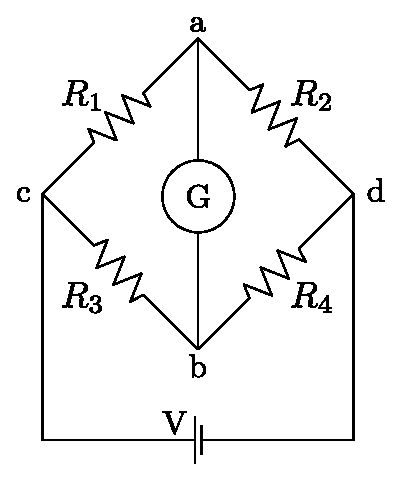
\includegraphics[scale=0.75]{resources/figura2.eps}
        \end{figure}

    \end{enumerate}

\end{enumerate}
\end{document}

